\subsection{2\texorpdfstring{\textsuperscript{k}}{k}r analysis}\label{subsec:ld2kr}

Analysis performed with \(k\!=\!4\) and \(r\!=\!10\), for a total of \(2^4 \cdot
10 \!=\!160\) experiments.

The simulation configuration for this analysis, named ``LowDensity2kr'' can be
found in the \code{simulations.ini} file. The simulations have been run using
our \code{simulate.sh} script with the following command:
\begin{verbatim}
$ ./simulate.sh -s LowDensity -c LowDensity2kr
\end{verbatim}

First, we have verified that the range of values for the \code{maxCopies}
parameter (2--6) was fine. The analysis can be found in \code{histograms.ipynb}.

Then, the 2\textsuperscript{k}r analysis can be found in \code{2kr.ipynb}. We
will verify the assumptions of normality, independence and finite variance for
the residuals in \secref{subsec:ldassumptions}. Here we will discuss the
results.

\section{Coverage}\label{sec:startnodecoverage}

File \code{coverage.ipynb} contains the histograms for the coverage obtained
with the configuration named ``StartNodePosition''. All parameters have been
fixed and we have performed 200 experiments with the starting user at the
center, border and corner --- for a total of 600 experiments.

The notebook also shows statistics about the coverage in the three cases.
Results are shown in \tableref{table:startnodecoveragestats}.

\begin{table}[hbt]
	\centering
	\begin{tabular}{lcccc}
		\toprule
		Start Node Pos\@. & Mean & Std\@. Dev\@. & Min\@. & Max\@. \\
		\midrule
		Center & \makecell[c]{\(1235.785\) \\ (\(98.942\%\))}
		       & \makecell[c]{\(7.084471\) \\ (\(0.5672\%\))}
		       & \makecell[c]{\(1213\) \\ (\(97.1177\%\))}
		       & \makecell[c]{\(1248\) \\ (\(99.9199\%\))} \\[16pt]
		Border & \makecell[c]{\(1225.345\) \\ (\(98.1061\%\))}
		       & \makecell[c]{\(123.317566\) \\ (\(9.8733\%\))}
		       & \(0\)
		       & \makecell[c]{\(1248\) \\ (\(99.9199\%\))} \\[16pt]
		Corner & \makecell[c]{\(910.64\) \\ (\(72.9095\%\))}
		       & \makecell[c]{\(546.580205\) \\ (\(43.7614\%\))}
		       & \(0\)
		       & \makecell[c]{\(1248\) \\ (\(99.9199\%\))} \\
		\bottomrule
	\end{tabular}
	\caption{Statistics about coverage when the starting node is in the
	center/border/corner (low density
	condition)}\label{table:startnodecoveragestats}
\end{table}

As we can see, the mean is higher if the starting user is positioned in the
center and lower if it is positioned in the border or corner. Additionally we
have higher standard deviations when the starting user is moved near the corner.
When the starting user is in the center, we have are able to guarantee a
coverage of at least \(97\%\) with \(R\!=\!25m\) in low density conditions,
while when the starting user is placed at the border or the corner the coverage
can drop down to zero.

Files \code{\{low,high\}-density-coverage.ipynb} contain the analysis of the
coverage in the two conditions (low density and high density) when the radius is
varied from very low values to high values. Data has been collected using the
configurations named ``StartNodePositionLowDensity'' and
``StartNodePositionHighDensity''.

\figref{subfig:ldstartnodecoverage} shows the results for the low density
case\footnote{For easier visualization, the Jupyter notebook also contains the
same data plotted in three different figures rather than with the center, border
and corner cases in the same plot.}. As we can see, in the ``center'' case the
mean coverage starts very high even with low values of \(R\): The minimum mean
is around \(1150\) (from a total of \(1249\) reachable users) and it stabilizes
near the value \(1240\) for \(R \ge 25m\).

\begin{figure}[hbt]
	\centering
	\begin{subfigure}[b]{0.49\textwidth}
		\centering
		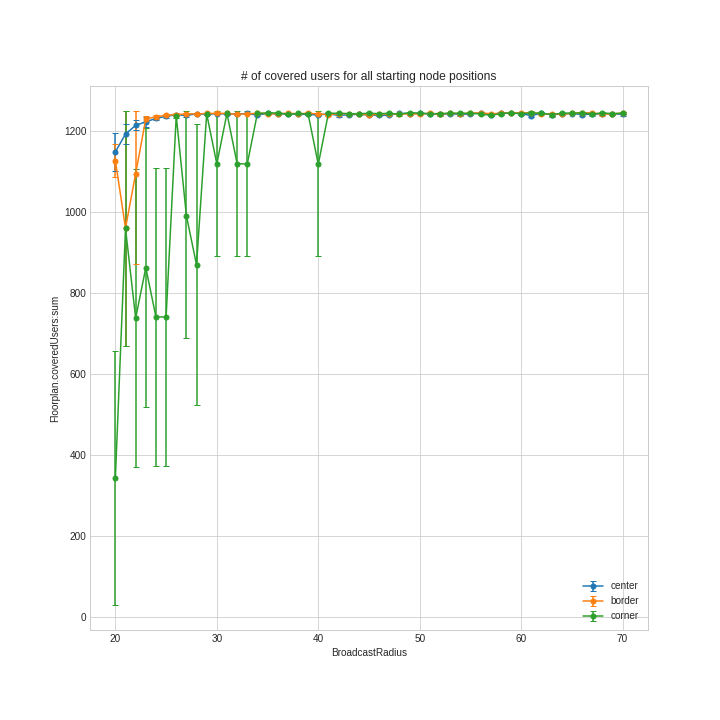
\includegraphics[width=\textwidth]{img/ld/start-node-coverage}
		\caption{Low density scenario}\label{subfig:ldstartnodecoverage}
	\end{subfigure}
	\begin{subfigure}[b]{0.49\textwidth}
		\centering
		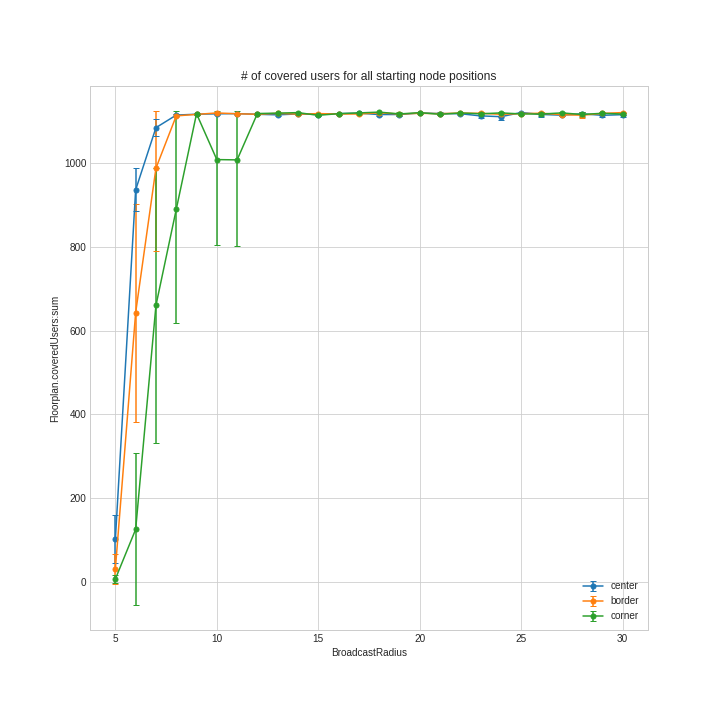
\includegraphics[width=\textwidth]{img/hd/start-node-coverage}
		\caption{High density
		scenario}\label{subfig:hdstartnodecoverage}
	\end{subfigure}
	\caption{For low values of \(R\), the coverage is generally worse if the
	starting node is in the corner rather than in the
	center}\label{fig:startnodepositioncoverage}
\end{figure}

Also in the ``border'' case the coverage stabilizes at high values with \(R \ge
25m\), but it has very high variance when the broadcast radius is very low and
it also happens that the first user sending the message is not able to reach
anyone, giving a coverage of zero.

In the ``corner'' case the situation is even worse: up until \(R \le 33m\) we
do not have a stable coverage and even after we get lower mean with a huge
variance with \(R\!=\!40m\). As we can see from the table at the end of the
notebook, this is due to a catastrophic experiment where the starting user has
not reached any user even with \(R\!=\!40m\).

\figref{subfig:hdstartnodecoverage} shows the results for the high density
scenario. Considerations are the same done for the low density scenario, so we
will not discuss the results here.

So, if possible, when designing a network of this type, to guarantee a nearly
perfect coverage, we should try to ensure that the starting user is near as much
as possible to the center or, at least, avoid the corners of the floorplan. If
this is not possible, to guarantee\footnote{With ``guarantee'' we do not mean a
100\% guarantee, of course: more experiments are needed to explore more
possibilities and, with the total randomness on the position of the users, the
only values of the broadcast radius that \emph{really} guarantees a coverage
greater than zero are those values that always make the starting user to reach
the entire floorplan immediately. Values found (\(40m\) and \(11m\)) are only an
\emph{hint} of minimum values that makes \emph{hard} to get a catastrophic
situation.} the coverage, it is necessary to increase the broadcast radius (\(R
> 40m\) for low density; \(R > 11m\) for high density).

The probability to found a user inside the area of reachability of the starting
node \idest{the probability to get a coverage greater than 0} can be easily
computed, in the general case, with~\eqref{eq:nocatastropheprobability}. The
equation has been derived by considering the inverse of the probability to found
\idest{the probability to \emph{not} found any node in the area of reachability,
which is the probability to found all the nodes in the area outside the area of
reachability} which is, for a single user, the area outside of the area of
reachability (\(X\cdot Y - \alpha\cdot\pi\cdot R^2\)) divided by the area of the
floorplan (\(X\cdot Y\)). This probability has been then extended to the case of
\(N\) users by raising it to the number of users except the first one (\(N-1\)).

\begin{equation}\label{eq:nocatastropheprobability}
	P = 1 - {\left(\frac{XY - \alpha\pi R^2}{XY}\right)}^{N-1}
\end{equation}

We can verify that for \(R\!=\!40m\), \(N\!=\!1250\), \(X\!=\!Y\!=\!500m\), with
the starting node in the corner (\(\alpha\!=\!\frac{1}{4}\)), we get:

\[
	P = 1 - {\left(\frac{500\cdot500 -
	\frac{1}{4}\pi\cdot40^2}{500\cdot500}\right)}^{1249} \simeq 99.81\%
\]

which is a quite high probability. Only in just \(\frac{1}{500}\) cases we will
get a coverage equal to zero in the case of the low density scenario with
\(R\!=\!40m\).

\subsubsection{Total number of collisions}\label{subsubsec:rect2krcollisions}

For the total number of collisions we get a very low unexplained variation
(\(0.72\%\)). The broadcast radius accounts for the \(64.31\%\) of the variation
and it is the dominant factor, as in other scenarios. As in the low density
scenario and differently from the high density one, the second most important
factor was the maximum number of copies, which accounts for the \(16.47\%\) of
the variation while the maximum relay delay (third factor) accounts only for the
\(4.86\%\) of the variation. In this case, also the combination of the broadcast
radius and the maximum number of copies is relevant (\(9.59\%\)). This results
are not surprisingly because the density of the rectangular scenario is the same
as the low density one (which is a square).

As in the case of other configurations, we need to decrease the broadcast radius
to reduce the total number of collision, which is an obvious consideration, and
as shown in \figref{fig:rectperfcollisionsm} using lower values for the maximum
number of copies reduces the total number of collisions.

The fact that the broadcast radius is less important in this scenario compared
to the high density case, but more important with respect to the low density,
can be explained by the fact that the users are scattered in the floorplan, so
we need a huger increase of the broadcast radius to see an effect, but they are
not so well distributed because they are flattened in the rectangle.

\begin{figure}[htb]
	\centering
	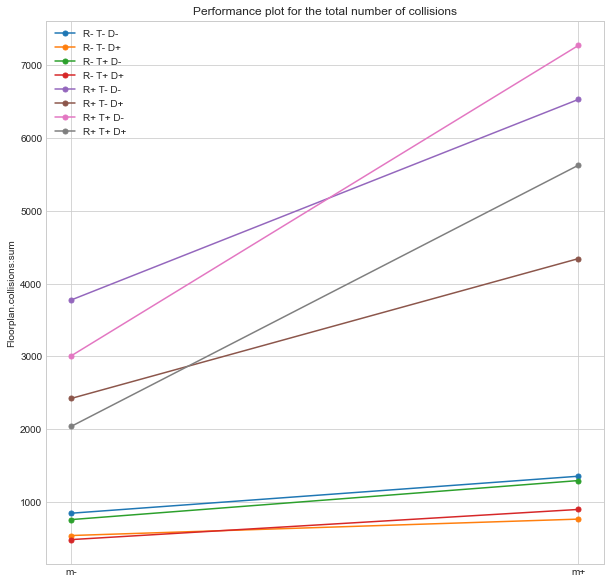
\includegraphics[width=\textwidth]{img/rect/collisions_m_perfplot.png}
	\caption{Decrease the maximum number of copies to decrease the total
	number of collisions}\label{fig:rectperfcollisionsm}
\end{figure}

\subsubsection{Total number of messages sent}\label{subsubsec:hd2krmessages}

This is an indication of the energy efficiency of the entire network.

The maximum number of copies is the dominant factor (\(85.98\%\)), as expected.
Also the broadcast radius \(R\) and its combination with the maximum
number of copies have a valuable impact on this index. The unexplained variation
is very low (\(0.53\%\)).

In \figref{subfig:hdperfmessagesm} we see that the total number of messages sent
decreases with an lower value of the \code{maxCopies} parameter, as expected.
We note that with \(m\!=\!6\) we get that nearly all the users of the network
relay the message. In \figref{subfig:hdperfmessagesR} we can see that less
messages are sent if an higher broadcast radius is used when \(m\!=\!2\). So,
with a low \(m\), we can further decrease the total number of messages sent by
increasing \(R\). Of course increasing the broadcast radius is not good for our
purpose to optimize the energy efficiency of the network, but as we can see from
\figref{subfig:hdperfmessagesT}, the same consideration made for \(R\) are also
valid for the hear window size \(T\). We perhaps expect \(T\) to hugely affect
the total broadcast time, so the selection of the factor \(T\) is a trade-off
between the energy efficiency and the total broadcast time.

\begin{figure}[hbt]
	\centering
	\begin{subfigure}[b]{0.33\textwidth}
		\centering
		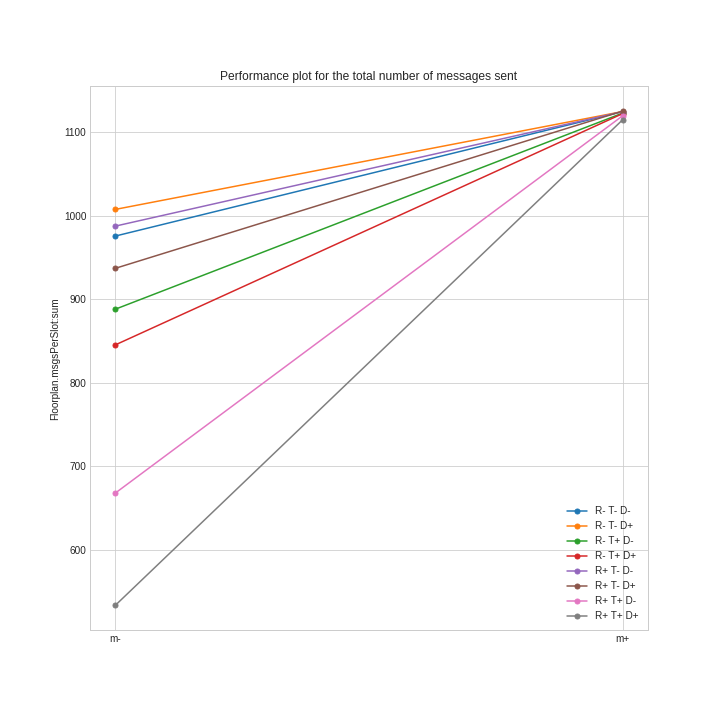
\includegraphics[width=\textwidth]{img/hd/messages-m-perfplot}
		\caption{When the maximum number of copies is reduced the total
		number of messages sent decreases}\label{subfig:hdperfmessagesm}
	\end{subfigure}
	\begin{subfigure}[b]{0.33\textwidth}
		\centering
		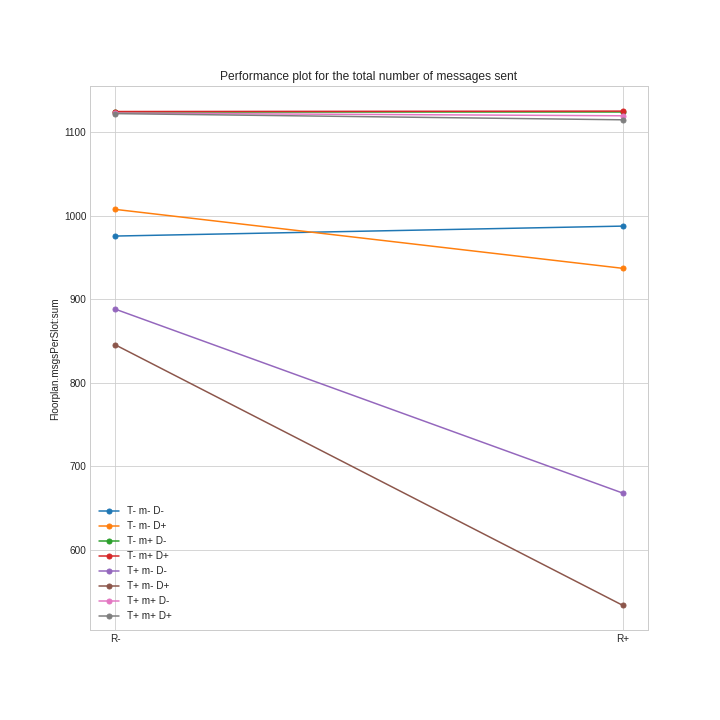
\includegraphics[width=\textwidth]{img/hd/messages-R-perfplot}
		\caption{Increase the broadcast radius when \(m\) is low to
		reduce the total number of messages
		sent}\label{subfig:hdperfmessagesR}
	\end{subfigure}
	\begin{subfigure}[b]{0.32\textwidth}
		\centering
		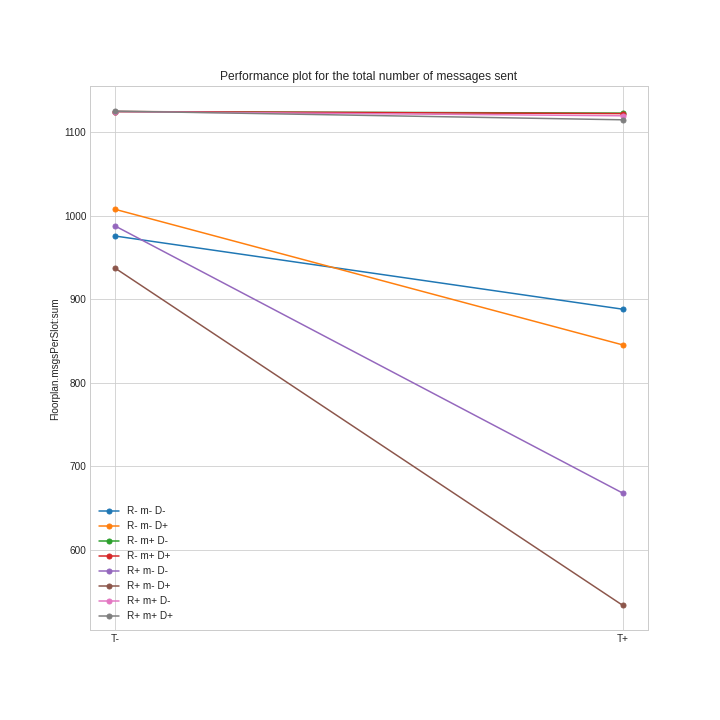
\includegraphics[width=\textwidth]{img/hd/messages-T-perfplot}
		\caption{Increase the size of the hear window when \(m\) is low
		to reduce the total number of messages
		sent}\label{subfig:hdperfmessagesT}
	\end{subfigure}
	\caption{Performance plots for the total number of messages
	sent}\label{fig:hdperfmessages}
\end{figure}

\subsubsection{Broadcast time}\label{subsubsec:hd2krtime}

Since in all the experiments we have always reached a coverage of at least
\(99\%\), here we will only discuss the broadcast time needed to reach the 99th
percentile of the coverage.

We have a large unexplained variation (\(7.95\%\)). The reason for this result
will be discussed in \chref{ch:starting-node}.

We can see that the most important factor is the broadcast radius that accounts
for the \(71.25\%\) of the variation, followed by the size of the hear window
(\(19.30\%\)). Other factors and their combinations are irrelevant. We note that
these variations are much larger than the unexplained variation, so we can still
say that they are significant. Of course, their \(95\%\) confidence intervals
also gets larger: (\(63.62\%\), \(79.30\%\)) for \(R\) and (\(15.43\%\),
\(23.59\%\)) for \(T\), but they do not include the zero.

This means that we can reduce the broadcast time by increasing the broadcast
radius to let the relayed messages to reach more user. Also the size of the hear
window can be decreased in order to reduce the time that each user wait before
deciding to relay or not relay the message. Of course, as stated before,
reducing the size of the hear window has a negative impact on the energy
efficiency, so some trade-off considerations are required.

We note that we have performed a \emph{logarithmic transformation of the
predicted variable} \idest{the total broadcast time} in order to meet the
assumption of finite variance for the residuals, as discussed in
\secref{subsec:hdassumptions}. This means that the final approximated regression
model for the broadcast time is transformed into the one shown
in~\eqref{eq:hdtimelogregressionmodel}, with \(R\) and \(T\) normalized between
\(-1\) and \(1\). (factors with low influence are removed; 95\% confidence
intervals are show in parenthesis).

\begin{equation}\label{eq:hdtimelogregressionmodel}
	\begin{cases}
		\log(t_B) = q_0 + q_R \cdot R + q_T \cdot T + e\\
		q_0 = 4.782874\\
		q_R = -0.462452 & (-0.487897, -0.437006)\\
		q_T = 0.240663 & (0.215217, 0.266109)
	\end{cases}
\end{equation}

We can then predict the total broadcast time using the formula shown
in~\eqref{eq:hdtimeregressionmodel}.

\begin{equation}\label{eq:hdtimeregressionmodel}
	t_B = e^{4.782874 - 0.462452 \cdot R + 0.240663 \cdot T}
\end{equation}

And the 95\% confidence interval as shown in~\eqref{eq:hdtimeregressionci}.

\begin{equation}\label{eq:hdtimeregressionci}
	\begin{cases}
		t^-_B = e^{4.782874 - 0.487897 \cdot R + 0.215217 \cdot T}\\
		t^+_B = e^{4.782874 - 0.437006 \cdot R + 0.266109 \cdot T}\\
	\end{cases}
\end{equation}

